\scanpage{4}
\reversemarginpar
\textcircled{\small 20} Vanishing theorem.\tikz[overlay,x=1em,y=1ex]{\fill (-.75,-1.1) circle (.45pt);} Cas des espaces homogènes.

\textcircled{\small 21} $H^{*}(X,F)\to H^{\unsure{*|x}}(X_{0},F_{0})$ ($X_{0}$ fermé dans $X$\tikz[baseline=(et.base)]{\node[inner sep=1pt] (et) {\inserted{ch. étale}};\draw (et.south west) .. controls +(0,-.1) and +(-.15,0) .. ([yshift=-3pt]et.south) -- ([yshift=-7pt]et.south) -- ([xshift=2pt,yshift=-3pt]et.south) .. controls +(.15,0) and +(0,-.1) .. (et.south east);}), quand est-ce un isom ? Suffit-il que ce soit vrai en dim $0$ ? Cas $X=\operatorname{Spec} A$, $X_{0}=\unsure{\operatorname{Spe}|\operatorname{Spec}|\operatorname{Sp}} A/J$, $A$ $J$-adique séparé complet. Cas de la localisation étale le long de $X_{0}\subset X$, $X$ affine.

22)\margin{travail Saavedra en train}% slanted
\hspace{.4em}Structure des catégorielles abéliennes avec produit tensoriel $\pm$ rigide, en termes de \unsure{représentation|représentations} linéaires des groupes proalgébriques, et de \unsure{représentation|représentations} de gerbes.... \inserted{(préliminaire algébrique à le théorie des motifs).}

\figure{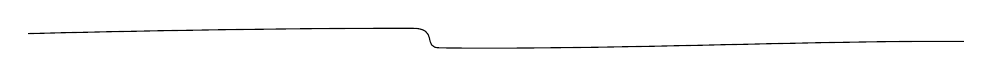
\begin{tikzpicture}[x=.98\linewidth,y=1ex]\draw (0,0) .. controls (.18,.35) and (.32,.45) .. (.41,.45) .. controls (.44,.45) and (.42,-1.2) .. (.44,-1.2) .. controls (.63,-1.35) and (.83,-.6) .. (1,-.65);\end{tikzpicture}}
\par\noindent\uline{Pour memoire}

\diagram{\resizebox{\linewidth}{!}{\begin{tikzcd}[ampersand replacement=\&,column sep=2.2em,row sep=0pt,cells={nodes={inner sep=0pt}}]
{\left.\begin{array}{@{}l@{}}
\otimes\ \text{Résolution des singularités.}\\[.8ex]
\otimes\ \text{Pureté cohomologique.}
\end{array}\right\}}
\arrow[r,Rightarrow,yshift=1.1em]
\arrow[r,Rightarrow,yshift=-1.2em]
\& {\begin{array}{@{}l@{}}
\text{dualité locale}=\text{bidualité,}\\[-.3ex]
\qquad\text{pour la top étale}\\[.8ex]
\text{th de finitude pour \unsure{morphisme|morphismes}}\\[-.3ex]
\qquad\text{\tikz[baseline=(fin.base)]{\node[inner sep=2pt] (fin) {\inserted{de type fini}};\draw ([yshift=-2pt]fin.north east) .. controls +(-.2,.05) and +(.2,0) .. (fin.north west) .. controls +(-.15,-.1) and +(-.1,0) .. (fin.south west) -- ([xshift=-8pt]fin.south east) .. controls +(.2,0) and +(0,-.1) .. (fin.north east);}}\\[-.3ex]
\text{etc etc}
\end{array}}
\end{tikzcd}}}

Changement de base régu\(\overset{\text{\scriptsize ?}}{\text{li}}\)er \inserted{en cohomologie.}

Dimension cohomologique des morphismes affines.

$\otimes$ \unsure{Théorème|Théorèmes} de finitude genre Grauert.

$\otimes$ Théories \deleted{\unsure{rig|rigide}} type rigide-analytiques.

Questions dans SGA 1962

\figure{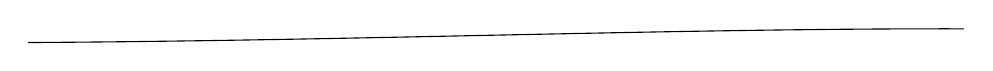
\begin{tikzpicture}[x=.98\linewidth,y=1ex]\draw (0,0) .. controls (.35,.15) and (.7,1.2) .. (1,1.15);\end{tikzpicture}}

\shortstack{23)\\[-.5ex]\scriptsize$\times$} Théorie de Chow pour Schémas \deleted{\unsure{qq|qcq} réguliers} ayant un faisceau inversible ample (équivalence rationnelle \unsure{des|de}\unsure{,} cycles). L'image inverse par $f:X\to Y$ doit être définie, sous seule condition que $Y$ soit régulier.

\tikz[baseline=(num.base)]{\node[draw,circle,inner sep=.7pt] (num) {\shortstack{24\\[-.5ex]\scriptsize$\times$}};}
\margin{Réponse négative Griffiths pour question 1\textsuperscript{o}}% slanted
\hspace{.4em}\inserted{1\textsuperscript{o}} Sur une variété projective lisse connexe de dim $3$ sur $k$ corps \unsure{algébriqmt|algébriquemt|algébriquement} clos, un $1$-cycle num. équiv. à $0$ est-il $\tau$-équivalent à zéro ? \inserted{En dim $4$, cycle de dim $2$ équiv. num $=$ équiv. hom ??\unsure{,|'}}
% archive sheet number: 3
\normalmarginpar

